\chapter{Plastic Omnium} \label{Plastic Omnium}

Plastic Omnium is a French automotive supplier specialized in 
The company is composed of two divisions that are both leader in their field of activity:


\begin{figure}
\centerline{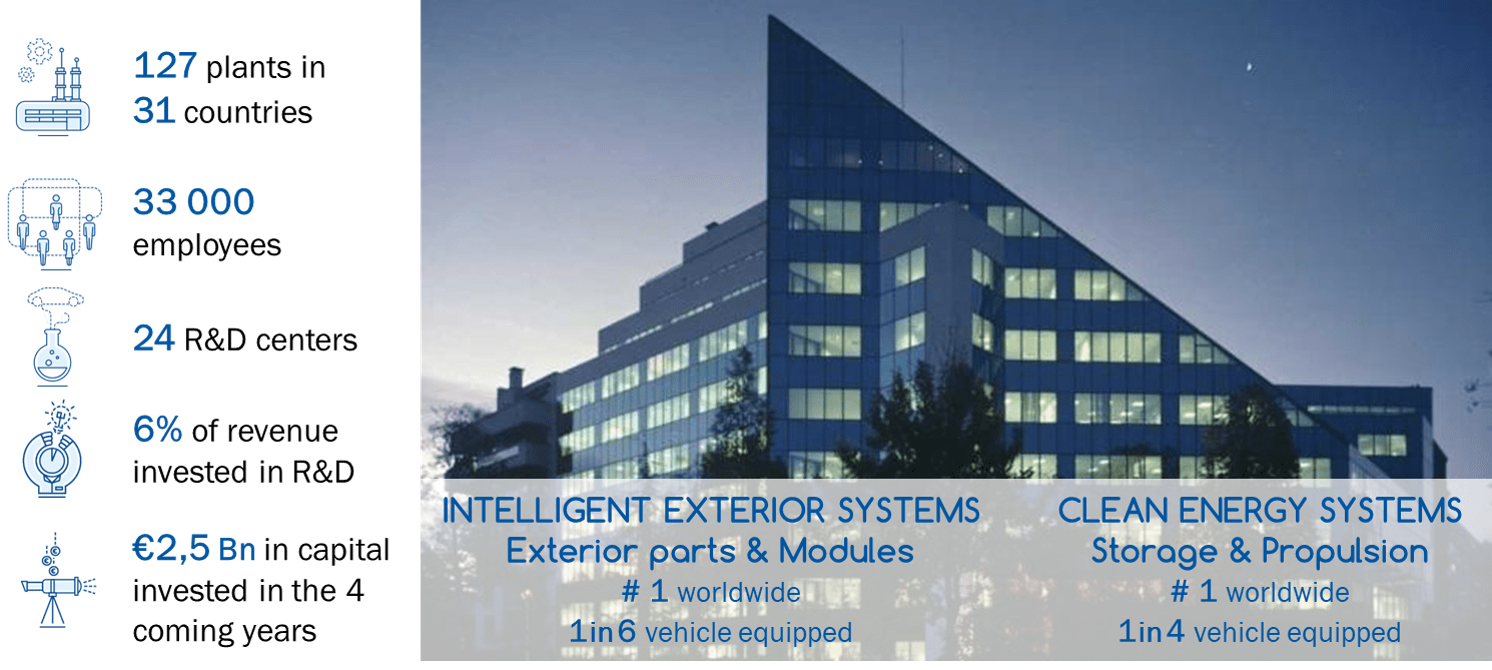
\includegraphics[scale=0.5]{images/appendix_A/PO_key_data.png}}
\caption{Plastic Omnium key data}
\label{fig:Plastic Omnium key data}
\end{figure}

%ADD image



\section{Clean Energy Systems}

The Clean Energy Systems (CES) division of Plastic Omnium is specialized in plastic fuel tanks systems, and depolluting systems, mostly for private and commercial vehicles. In 2018, more than 22M fuel systems have been delivered, representing 1 out of 4 commercialized vehicles equipped with a fuel system coming from the CES division.
The material used for producing the fuel tanks is HDPE (High-Density Polyethylene). There are several reasons why they are made of plastic and not in metal as they used to be (for cars):
\begin{itemize}
    \item Plastic is lighter than metal (about 30\%), which allows a reduction of fuel consumption.
    \item The raw material is less expensive.
    \item A plastic tank cannot explode: it will melt, and the fuel will be spilled on the floor.
\end{itemize}

However, one issue is the permeability: as plastic is a porous material, fuel will eventually end up going through it and that leads to two major issues: the consumer will lose some of his gas, and this one will go into the air and pollute the atmosphere. That is why a fuel tank is not a simple container of fuel: it’s a real part composed of complex technologies, from the production processes to the material used, and also the parts attached to the fuel system; filling system, pump gauge module, ventilation. These are used to make the fuel system (Figure \ref{fig:Fuel System}) less permeable to cope with the different regulations.
\begin{figure}
\centerline{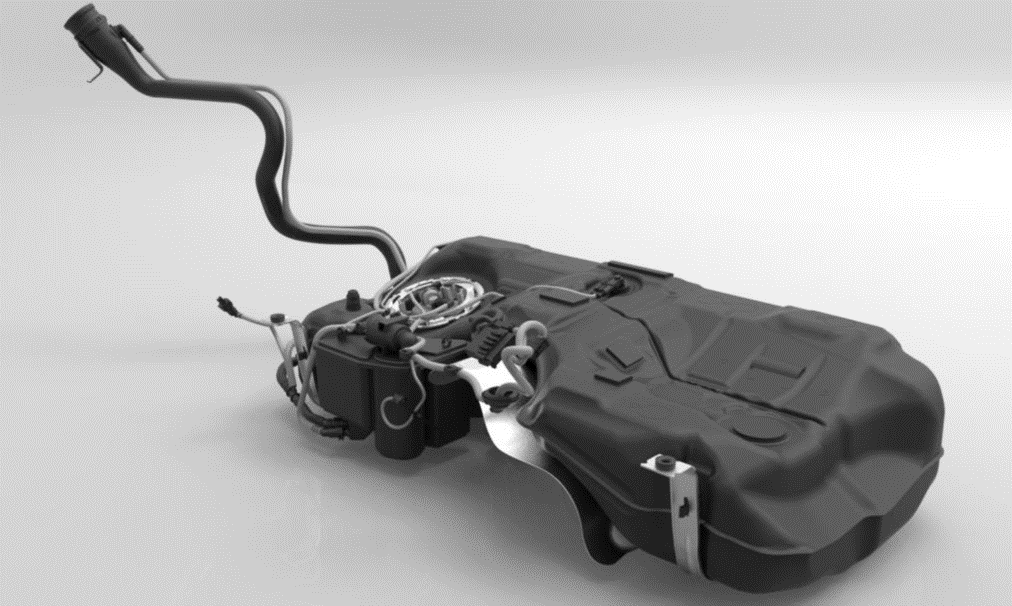
\includegraphics[scale=0.4]{images/appendix_A/fuel_system.png}}
\caption{Fuel System}
\label{fig:Fuel System}
\end{figure}
A fuel system is composed of a fuel tank (Figure \ref{fig:Plastic Fuel Tank}) and a filler pipe (Figure \ref{fig:Filler Pipe}, the latter is the only part visible of the system by the end user, to refill the tank at the station.

\begin{figure}
\centerline{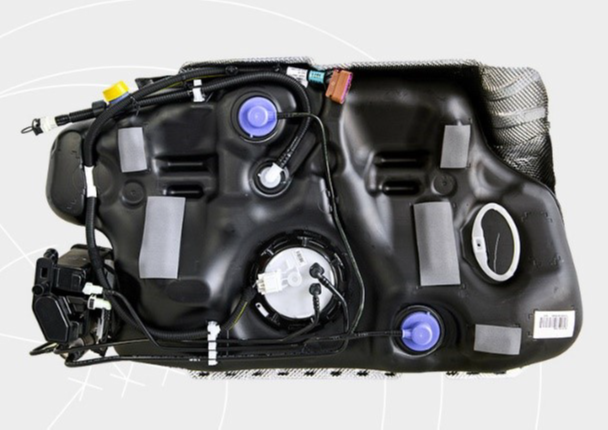
\includegraphics[scale=0.6]{images/appendix_A/Plastic_fuel_tank.png}}
\caption{Plastic Fuel Tank}
\label{fig:Plastic Fuel Tank}
\end{figure}
\begin{figure}
\centerline{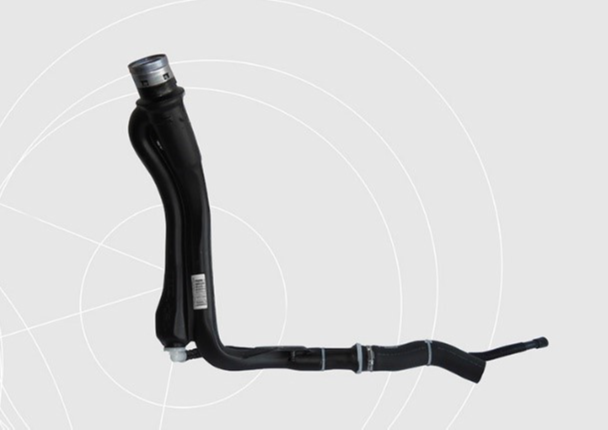
\includegraphics[scale=0.6]{images/appendix_A/Filler_pipe.png}}
\caption{Filler Pipe}
\label{fig:Filler Pipe}
\end{figure}

SCR technology is an effective response to the regulatory requirements limiting emissions of nitrogen oxides ($NO_x$) from diesel vehicles. Combining a tank with a pump and gauge module, this system injects vaporized \textit{AdBlue®} into the hot exhaust gases, causing a chemical reaction that transforms $NO_x$ into water vapor. Plastic Omnium has developed a range of SCR systems to meet the needs of all types of vehicles, from the smallest European city car to the largest American pickup truck.

\section{Intelligent Exterior Systems}

Intelligent Exterior Systems, IES, specializes in the manufacturing of complex car
body systems for car manufacturers. Examples of products are shown below: bumpers and
energy absorption systems, fender modules, front-end assemblies and rear-closure modules.

Today’s tailgate on boards state-of-the-art technology, customized and adapted to each customer requirements: plastic structure reinforced with metal or composite inserts, glued painted skin and local reinforcements to meet crash requirements.
Plastic Omnium designs also a range of exterior parts (fender flares, rocker panels, door trims) that add to the esthetic and distinctive character of the vehicles from each automaker.

\section{New Energies}

The \textit{New Energies} division, born in 2021, aims to contribute towards hydrogen-powered electric mobility. As part of the European H2HAUL project intended to deploy hydrogen mobility in road transport, the New Energy division has just produced vessels at its Herentals (Belgium) site. 

\begin{figure}
\centerline{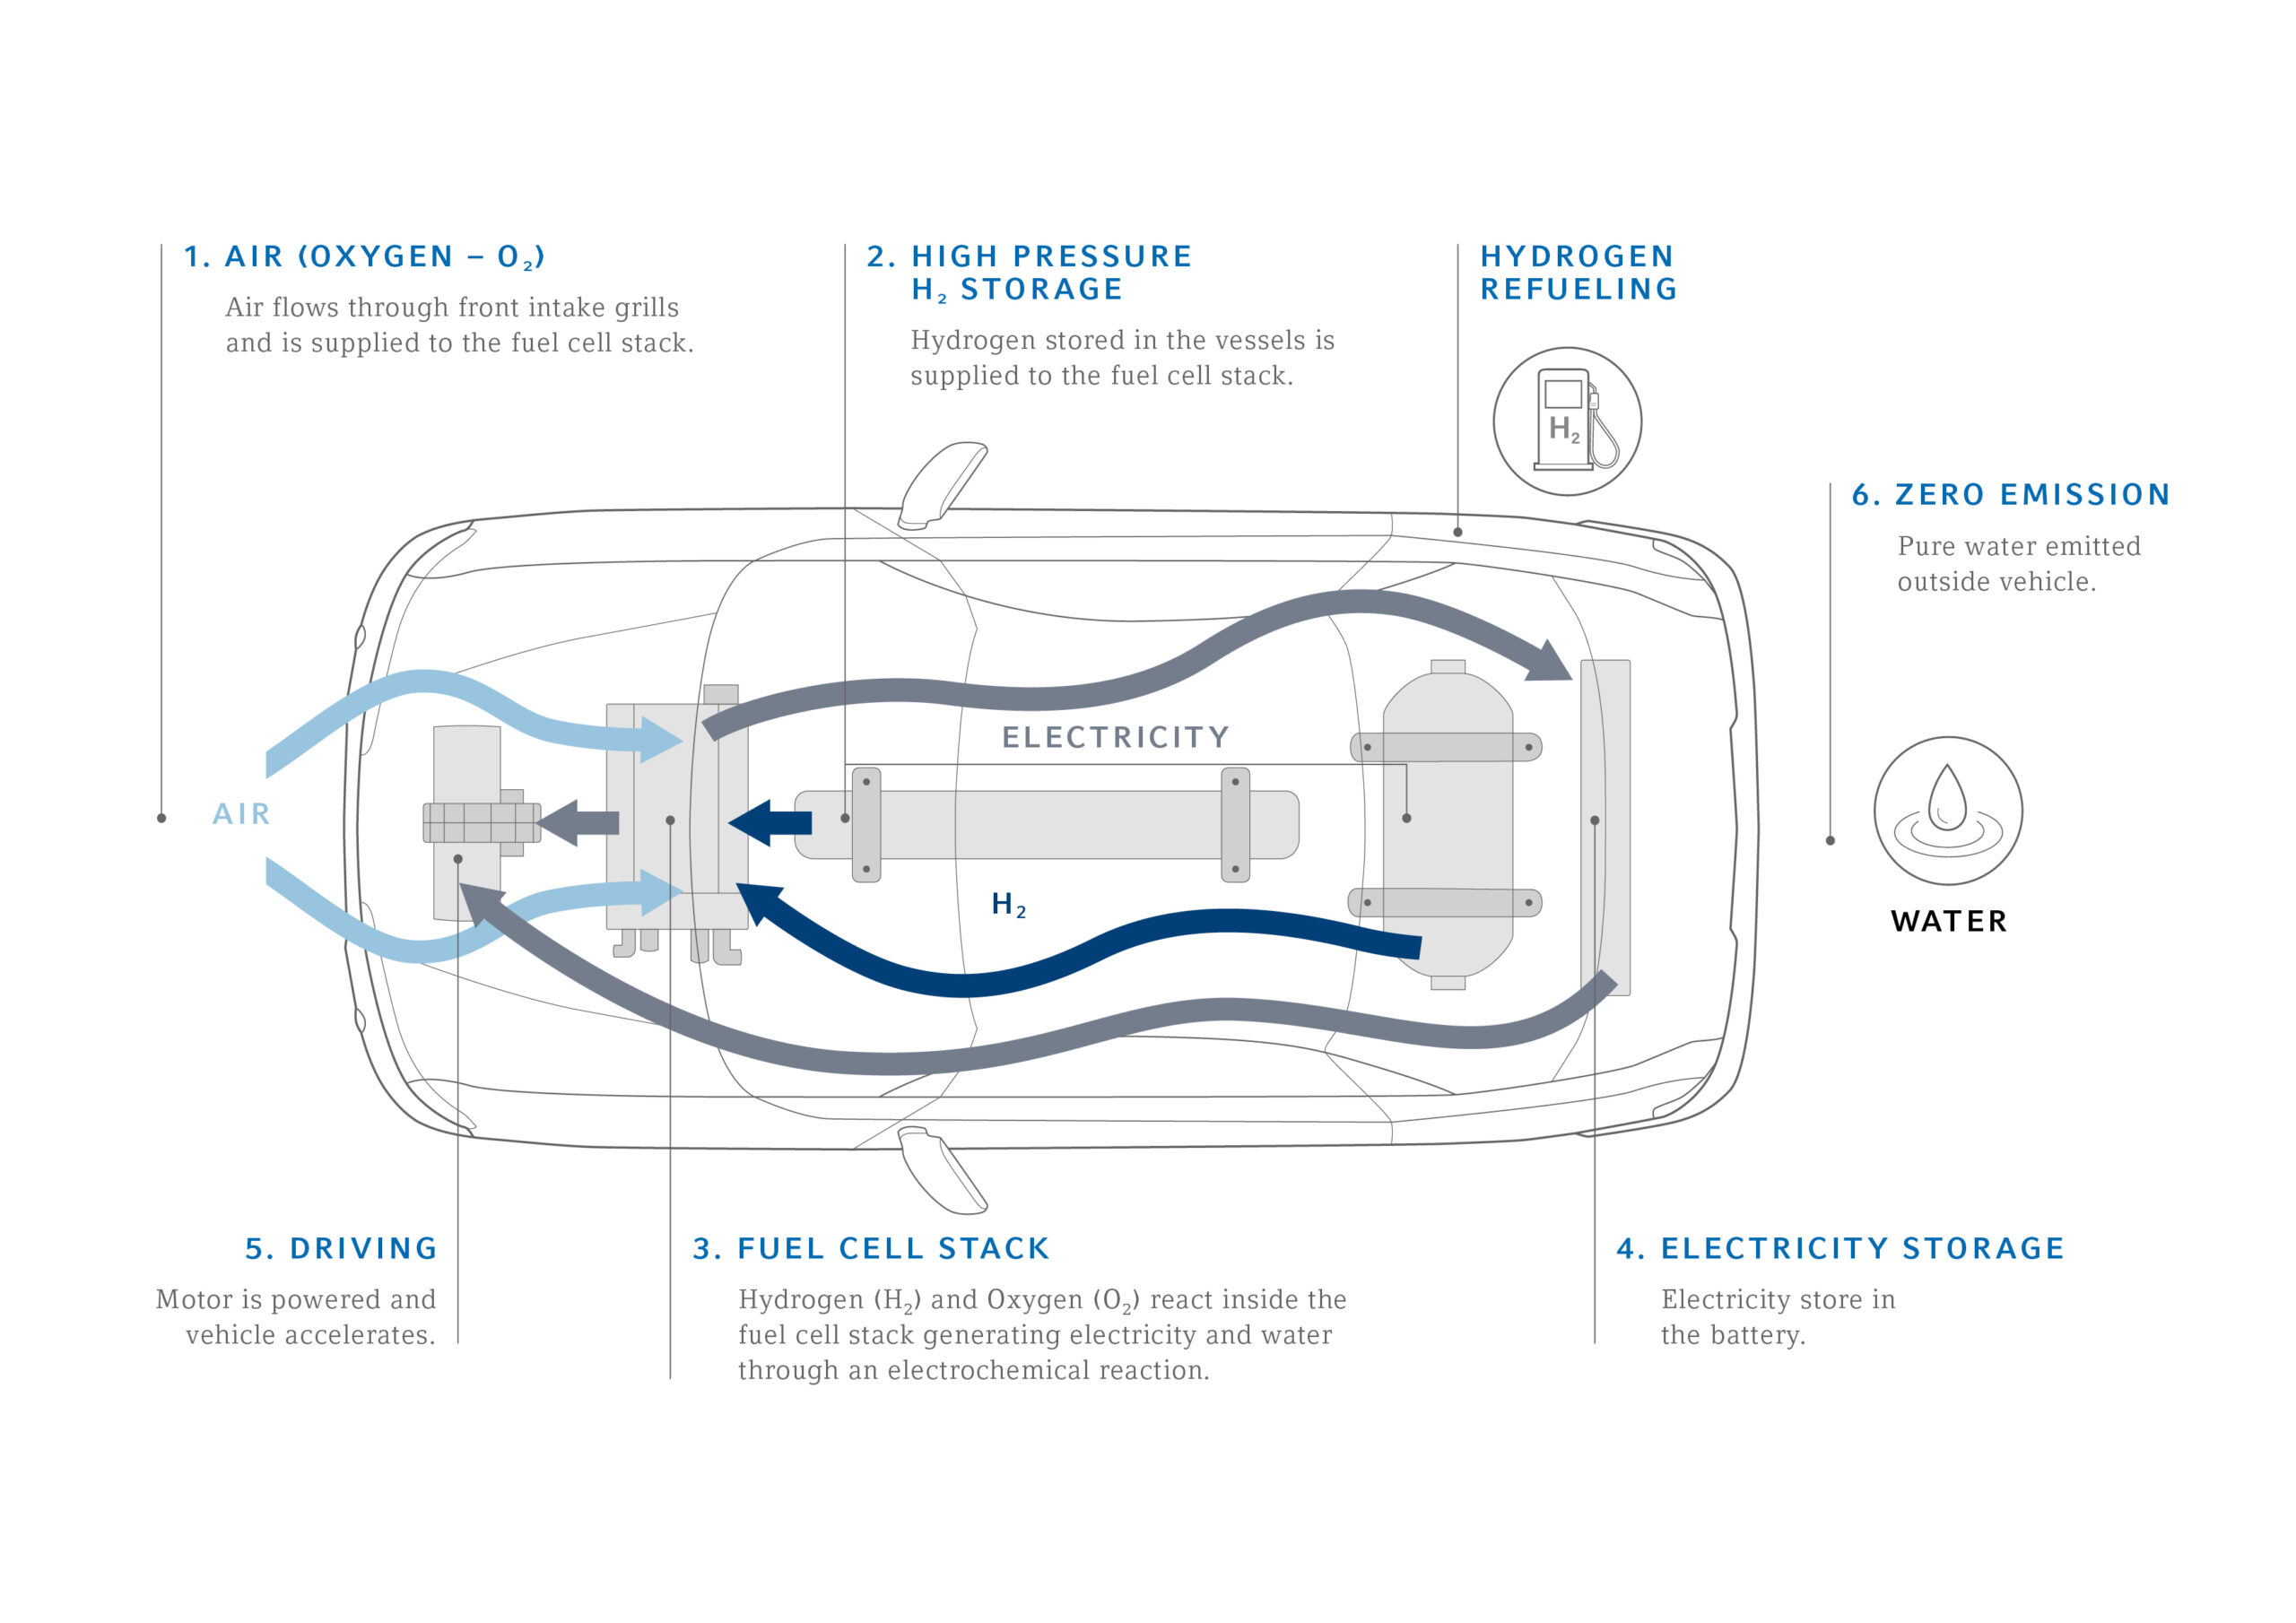
\includegraphics[scale=0.2]{images/appendix_A/plastic-omnium-voiture-zero-emission-legendes-scaled.jpg}}
\caption{Plastic Fuel Tank}
\label{fig:Plastic Fuel Tank}
\end{figure}
